\documentclass[11pt,onecolumn]{article}
\usepackage[margin=2.3cm]{geometry}
\usepackage{program}
\usepackage{graphicx}
\usepackage{listings}
\title{Sindice Dataset Summary and Assisted SPARQL Query Editor}
\author{Thomas Perry\\School of Computational Science \& Engineering\\ Georgia Institute of Technology\\ thomas.perry@deri.org}

\newcommand{\tab}{\hspace*{2em}}
\begin{document}
\normalsize
\maketitle


\section{Introduction}
The Sindice Dataset Summary is a class-based summary of the Sindice-2011 Dataset.  Currently when exploring a dataset through Sindice Search, a user must explore entity-level structured and semi-structured data to understand the the vocabulary and data model within it.  However, many entities have a class definition (e.g. foaf:Person, foaf:Organization, etc.) which can be used to provide a high-level overview of the dataset.  In the Sindice Dataset Summary, all entities of the same class are represented by a super-node with the same class definition and their aggregated properties.  Entities without a class definition as well as literal values are not represented in the summary.  Consider a dataset using the FOAF vocabulary and containing a list of academics, the organizations to which they belong, and their publications (See figure 1).  This dataset will be referred to as academic-dataset.org.  

\begin{figure}
  \centering
    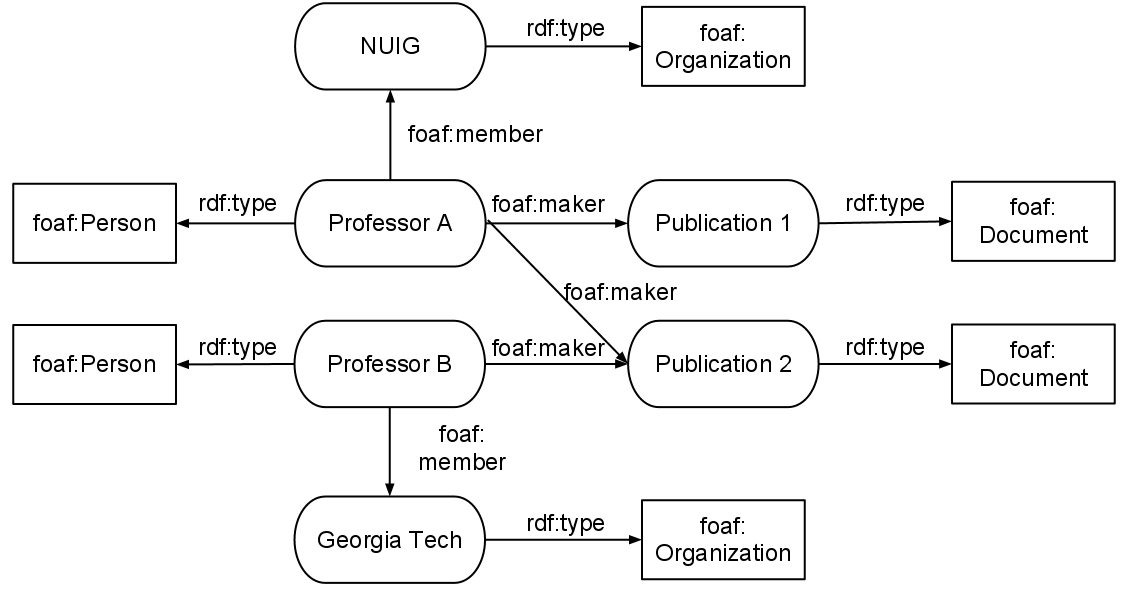
\includegraphics[width=0.6\textwidth]{Diagram1.png}
    \caption{Academic Dataset}
\end{figure}

The summary of this academic-dataset.org would consist of three super-nodes of class foaf:Person, foaf:Document, and foaf:Organization.  These super-nodes would have the properties, foaf:Person foaf:member foaf:Organization and foaf:Person foaf:maker foaf:Document.  This high-level overview allows users to quickly understand the vocabulary through the most common classes and relationships within a dataset without inspecting entity-level data.  This summary provides information that could also be used to assess dataset relevance to a query, assess dataset quality, assist in dataset exploration and recommendation, and assist in computing the shortest path between entities of class.  The Sindice Dataset Summary can also be integrated into other applications such as the Sindice Assisted SPARQL Query Editor.
 

\begin{figure}
  \centering
    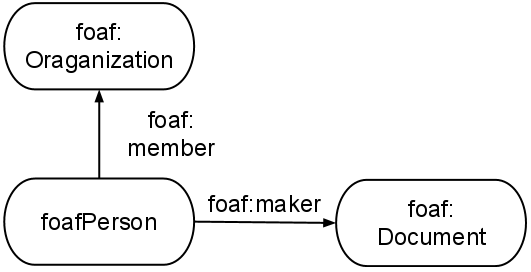
\includegraphics[width=0.40\textwidth]{Diagram2.png}
    \caption{Class-based Summary of Academic Dataset}
\end{figure}



In this part we focus on the problem and recommendation and explanation based the Sindice Assisted SPARQL Query Editor.  The Sindice Assisted SPARQL Query Editor is a SPARQL query editor which leverages the Sindice Dataset Summary to help users more effectively write SPARQL queries. The editor assists the user by  providing the most common properties and classes within a specified dataset.  The editor also provides in-query context-aware schema type recommendations.  Continuing with the academic dataset previously introduced, if a user requests a class recommendation within this dataset, the editor would only recommend the classes foaf:Person, foaf:Document, and foaf:Organization.  When recommending a property between entities of class foaf:Person and foaf:Document, the editor would recommend the property foaf:maker.  Thus the actual data being queried powers the editor's recommendations.


The remainder of this paper addresses the technical challenges of computing the Sindice Dataset Summary and implementing the Sindice Assisted SPARQL Query Editor.  Section 2 addresses background information that us relevant to understanding these challenges.  Section 3 covers the implementation of the Sindice Dataset Summary and Section 4 covers the implementation of the assisted query editor.  Section 5 discusses experimental results and section 6 covers the conclusion and future work.

\subsection{Contribution}
We study the computational steps required to compute a class-based summary of the web of data and how to leverage this information in an assisted SPARQL query editor.

ADD MORE HERE

\section{Background}
This work is a technical report on the computational methods used to analyze the Sindice Dataset[1], which is a reflection of the current Web of Data.  The Sindice dataset is a continually growing and updated dataset. The dataset contains nearly 15 billion statements from 423 million documents that correspond to 3.7 billion entities as of 10/11/2011.  Additional statistics concerning the Sindice Dataset are found in Table 1.

\begin{table}[h!]
\begin{center}
  \begin{tabular}{| l | r | }
    \hline
    {\bf Statistic}   & {\bf Description} \\ \hline
    Second-level Domains & 350,284 \\ \hline
    Total Documents & 423,529,552 \\ \hline
    Entities & 3,692,718,997 \\ \hline
    Total Explicit Triples & 14,906,282,573 \\ \hline
  \end{tabular}
 \caption{Sindice Dataset Statistics}
\end{center}

\end{table}

GET RECOMMENDATIONS FOR BACKGROUND INFO


\section{Dataset Summary Model}
The Web of Data is a set of datasets.  These datasets can be represented as a graph, $G$, which consists of nodes, $V$, and edges, $A$.  The nodes represent entities while the edges represent relationships among nodes. Let $P$ be the set of predicates. An edge, $a \in A$, is defined as a triple, $(e,p,v) \in V_E \times P \times V$.  Let $Z$ represent the set of all second-level domains within the Sindice Dataset.

The nodes $V$, can be partitioned into two disjoint sets.
\begin{itemize}
  \item $V_E$ the set of entity nodes (i.e. URI or blank nodes).
  \item $V_L$ the set of literal nodes,the attributes of an entity (i.e. literals).
\end{itemize}\\


Let $L$ be a set of labels, that can be distinquished:
\begin{itemize}
  \item $L_V$ the node labels
  \item $L_A$ the edge labels
\end{itemize}\\


The Web of Data can be modelled as the tuple $G =<V,A,\omega>$, where $\omega$ is a node labelling function $\omega: V \rightarrow L_V$.  The set of labelled edges $A$ can be defined as $\left\{ (e,a,v) \mid e \in V_E, a \in L_A, v \in V \right\}$.



We define the function $\gamma: V \rightarrow Z$. When $v \in V$ is a URI, $z$ is the second-level domain of the URI.  When $v \in V$ is a blank node or literal, $\gamma$  maps $v$ to the second-level domain of the document in which $v$ was published. We also define a function $\mu: A \rightarrow Z$.  $\mu$ maps an edge, $a \in A$, to the second-level domain of the document in which $a$ was published.


The nodes, $V$, can be partitioned into $\mid Z \mid$ disjoints sets, $V^z$, referred to as an abstract dataset.  One set for each second-level domain $z \in Z$.
\begin{itemize}
  \item $V^z$ the entities which are defined within the dataset $z$ (i.e. $\{e \in V \mid \gamma(e) = z \}$).
\end{itemize}\\

The edges, $A$, can be partitioned into $\mid Z \mid$ sets, $A^z$, referred to as a crawled dataset.  One set for each second-level domain $z \in Z$.
\begin{itemize}
  \item $A^z$ the edges which are published within the second-level domain $z \in Z$ (i.e. $\{ a \in A \mid \mu(a) = z \}$).
\end{itemize}\\
Please note the difference in the definitions of $V^z$ and $A^z$ with respect to the functions $\mu$ and $\gamma$.


A dataset $d$ is a tuple $d = < V^d, A^d, \omega >$ with $V^d \subseteq V$ and $A^d \subseteq A$. 



\\
{\bf Intra-dataset Edge}: an edge $(e,p,v)$ is said to be intra-dataset if $\gamma(e) = \gamma(v)$\\
{\bf Inter-dataset Edge}: an edge $(e_1,p,e_2)$ is said to be inter-dataset if $\gamma(e_1) \neq \gamma(e_2)$\\
{\bf Authoritative Edge}: an edge $a =(e_1,p,e_2)$ is said to be authoritative if $\gamma(e_1) \mbox{ or } \gamma(e_2) = \mu(a)$.\\
{\bf Non-Authoritative Edge}: an edge $a = (e_1,p,e_2)$ is said to be non-authoritative if  $\gamma(e_1) \mbox{ and } \gamma(e_2) \neq \mu(a)$..\\
\\
 
{\bf Entity Class Definition}: $ M^z(e) = \{ c \mid  a = (e, p, c ) \in A, \mu(a) = z = \gamma(e) , p \in \Psi \}$ where $\Psi$ is a finite set of predicates used to define a class.\\

{\bf Class Cardinality}: $C(M^z) = \mid \{ e \in V_E \mid M^z(e) = M \} \mid $\\

{\bf Class-edges}: $\{(M_1,p,M_2) \mid (e_1,p,e_2) \in A, M^{z_1}(e_1) = M_1, M^{z_2}(e_2) = M_2 \}$\\
{\bf Authoritative Class-edges}: $\{(M_1,p,M_2) \mid a =(e_1,p,e_2) \in A, M(e_1) = M_1, M(e_2) = M_2, \gamma(e_1) \mbox{ or } \gamma(e2) = \mu(a) \}$\\
{\bf Non-Authoritative Class-edges}: $\{(M_1,p,M_2) \mid a = (e_1,p,e_2) \in A, M(e_1) = M_1 , M(e_2) = M_2, \gamma(e_1) \mbox{ and } \gamma(e2) \neq \mu(a) \}$\\
{\bf Intra-Domain Class-edges}: $\{(M_1,p,M_2) \mid (e_1,p,e_2) \in A, M(e_1) = M_1,  M(e_2) = M_2, \gamma(e_1) = \gamma(e2) \}$\\

{\bf Inter-Domain Class-edges}: $\{(M_1,p,M_2) \mid (e_1,p,e_2) \in A, M(e_1) = M_1, M(e_2) = M_2, \gamma(e_1) \ne \gamma(e2) \}$\\


\subsection{Class Definitions}

For projects discussed within this document, we use an expanded definition $\Psi$, the properties used to define a class.  Typically an entity's class is only defined by the property rdf:type (http://www.w3.org/1999/02/22-rdf-syntax-ns\#type), $\Psi = \{\mbox{rdf:type}\}$.  The reason for the expanded definition is based on observations from the data within the Sindice Dataset.  Many datasets are defining classes with other properties than rdf:type, such as ogp:type and purl:type.  Specifically, Facebook's Open Graph protocol is extremely prevalent.  Nearly 80.82 million documents contain a class definition using a variation of the property ogp:type as compared to the 123.99 million documents using rdf:type.  While some datasets exclusively one property to define a class, some datasets use multiple properties to define a class.  For example, the dataset rottentomatoes.com as of 11/10/2011 used rdf:type to define the class dv:Movie (http://rdf.data-vocabulary.org/\#Movie) while using ogp:type to define the class “actor”.  If properties that define a class are limited to merely rdf:type, the class-based summary loses valuable information concerning the class "actor" in this dataset.  Without the expanded definition of $\Psi$, any dataset the exclusively used  properties other than rdf:type would be removed from the dataset summary.  Thus to expand the classes represented witin the summary, we expanded $\Psi$.

To expand the properties used to define a class, we selected several of the most common alternatives to rdf:type in the Sindice Dataset and properties specifically selected to improve the summarization of the Dbpedia dataset. The properties we included in $\Psi$ are the following:

\begin{table}[h!]
\begin{center}
  \begin{tabular}{| l | r | }
    \hline
    {\bf Property} & {\bf Documents in Sindice Dataset} \\ \hline    
    http://www.w3.org/1999/02/22-rdf-syntax-ns\#type & 123,994,777 \\ \hline
    http://opengraphprotocol.org/schema/type & 61,202,581 \\ \hline
    http://ogp.me/ns\#type & 17,184,227 \\ \hline
    http://opengraph.org/schema/type & 2,443,773 \\ \hline
    http://purl.org/dc/elements/1.1/type & 11,367,218 \\ \hline
    http://dbpedia.org/property/type & 120,044\\ \hline
    http://dbpedia.org/ontology/type & 65,796\\ \hline
  \end{tabular}
\end{center}
\caption{Properties that can define a class}
\end{table}



\section{Sindice Dataset Summary Implementation}

The Sindice Dataset Summary is a class-based graph summary of the Sindice-2011 Dataset.  In this summary, entities of the same class and within the same domain are represented by a super-node with the same class definition and their aggregated properties.  Compare the raw data of academic-dataset.org in Figure 1 with its summary in Figure2.  Entities without a class definition are not represented in the summary. This high-level overview allows users to quickly understand the vocabulary and the most common classes and relationships within a dataset without inspecting entity-level data.  This summary provides information that could also be used to assess dataset relevance to a query, assess dataset quality, assist in dataset exploration and recommendation, and assist in computing the shortest path between entities of class.  





\subsection{Computational Framework}

The Sindice Dataset is approximately 5 TBs of uncompressed data and 500 GBs compressed.  With this scale of data, it is necessary to utilize distributed computing.  The computational framework we utilized was Hadoop, an Apache open-source Java library for distributed computing on large datasets across a cluster of computers  Hadoop utilizes the MapReduce programming model and is designed to scale up from single servers to thousands of machines, each offering local computation and storage. Hadoop is designed to be fault tolerant, easily scalable, and abstract the user from low level message passing and scheduling.  MapReduce can be difficult to develop for, as such the Sindice Dataset Summary was developed using Cascading, a library providing an abstraction layer for Hadoop.

\subsection{Workflow}

The Sindice Dataset Summary computational workflow consists of five major steps.  The first step is to parse and prepare the data for processing.  The second step is to generate a table of the entity URI and their set of class.  The third step is to compute the frequency of each class within each dataset from the entity URI-class table computed in step 2.  Step four is to replaces the entities within the Sindice Dataset with their class definitions.  Step 5 is to aggregate the all the entities of the same class into a super-node of the same class definition. 

\begin{figure}
  \centering
    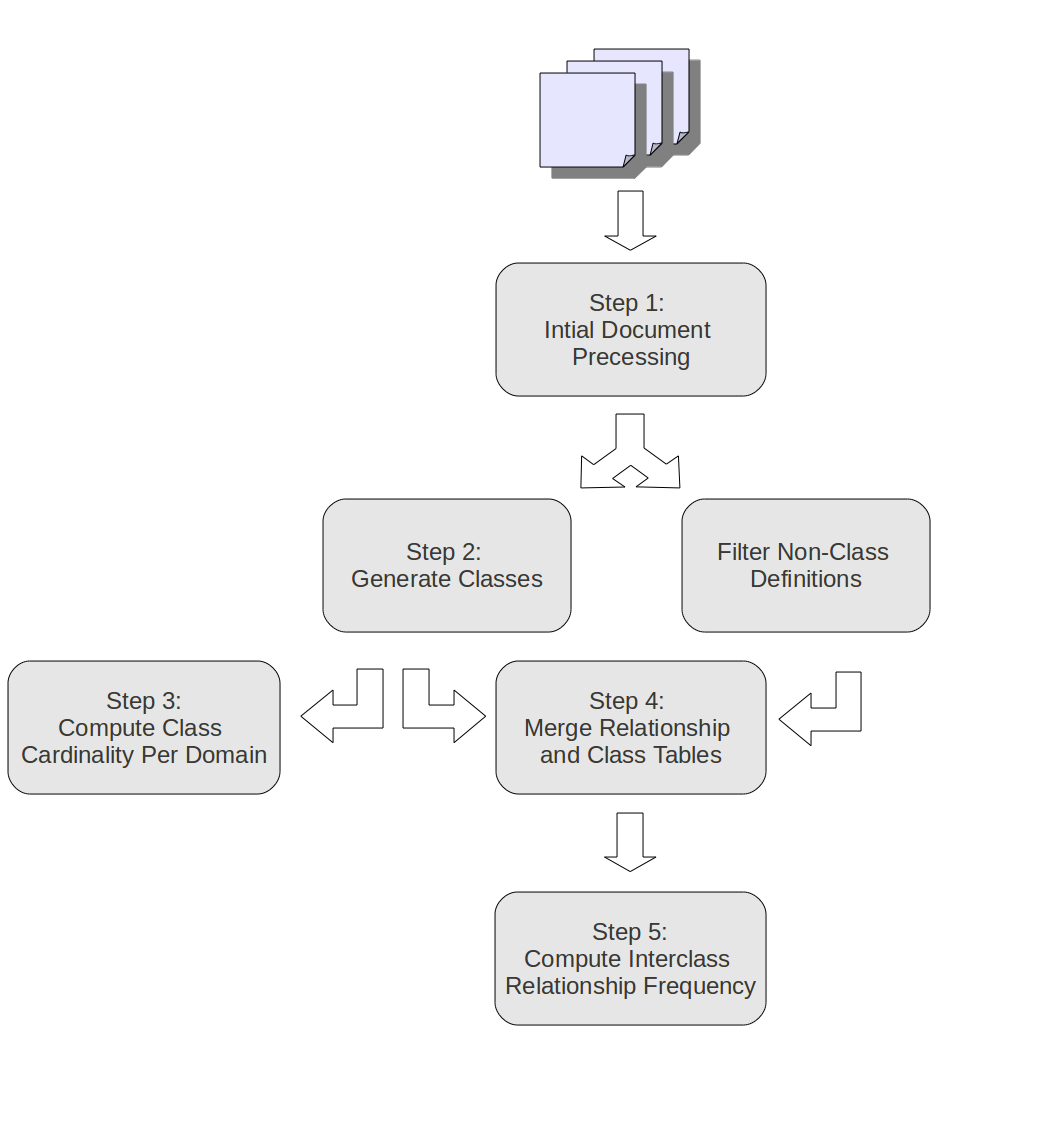
\includegraphics[width=0.55\textwidth]{workflow.png}
    \caption{Sindice Dataset Summary Workflow}
\end{figure}


\subsubsection{Step 1: Initial Document Processing}
Initial document processing prepares the raw data to be processed by the remainder of the workflow by performing three basic tasks. First is parsing, filtering, and normalizing the data.  Second is aggregating an entity's class definition at the document level.  Third is to compression.  The output of this stage is stored in a temporary directory for further processing by other stages.

\paragraph{Parsing, Filtering, Normalization}
\\
We remove as much initial data as possible to improve processing by following stages. As such, all non-authoritative class definitions are removed (see formal definition) as only authoritative class definitions are kept in our summary. All triples that define a class are aggregated into a single triple in which the object is the set of class definitions(for further explanation, see below).  Triples with containing literal values are removed except then they are a class definition.  The reason of removing literal values is they are unnecessary information because they will not be represented within the class-based summary. Triples that contain literal values that are a class definition are normalized. The literals are made lowercase, language tags are removed, and leading and trailing whitespaces are removed.  It is important to note that blank nodes are local identifiers and as such, the url of each blank node is prepended to its identifier.  This allows the summary to distinguish between two entities with the same blank node identifier but from different documents.  The output of this step is a record for each remaining triple that contains the domain in which it was published, its subject, predicate, object, and a flag indicating if the triple defines a class.


\paragraph{Aggregating Class Definition}
To reduce the number of records that will be sorted when generating the complete class definition for each entity, class definitions are first aggregated on the document level before over the entire Sindice Dataset.  While reading the triples within a document, for each entity, the triples that define the class are grouped together.  Then for each entity with a class definition, the set of class definitions are written to a single value, such as BytesWritable, that can later be parsed to extract the individual classes.  The set of triples defining the class set are removed are replaced a single triple with the same subject and predicate but now with the aggregated class definition for the object.  This step is very fast because it is performed locally because it occurs during map phase.  


\paragraph{Compression} \\
With the scale of data being processed, it is necessary to use compression to improve performance. Compression is not only useful for saving disk space, but it also maximizes IO throughput[example paper].  Java encodes strings in UTF-16, which represents each character with one or two 16-bit values.[http://rosettacode.org/wiki/String\_length\#Java].  When representing data as a String the byte size for each value is variable.  ADD STATISTIC ABOUT SIZE OF LITERAL.  To improve compression throughout the workflow, during this step, each URI and literal in the data is assigned a unique id.  The String value is removed and the remainder of workflow performs all computations on the unique ids. When the workflow is completed the unique ids are replaced with their String value.  To assign the unique id, we used the MurmurHash3 by Austin Appleby.  MurmurHash is optimized for hash-based look up and supports up to 128 bits.  When processing the raw data, each element in a triple is assigned an id by MurmurHash.  It is important to ensure that the correct length of hash is used.  If the hash is too short, relative to the number of ids being assigned, then different values will be assigned  the same id.  If this occurs, data can be lost or invalid. For example, two datasets could be assigned the same id (also referred to as a collision), as result they will be represented by single dataset in the summary that will contain the contents of both datasets.  If the hash is too long, this will reduce compression and IO throughput.   

The probability of a collision can be estimated by 
\begin{equation}
P_{collision} = 1-exp{\frac{-k(k-1)}{2N}}
\end{equation}

where k is the number of unique ids assigned out of N possible values [http://preshing.com/20110504/hash-collision-probabilities]. Initially we used 64 bit to hash hash entity URI, however $P_{collision}=0.309$ for 3.7 billion entities.  As such we used 128 bits, $P_{collision}=2.0\times10^{-20}$, which is equivalent to  8-16 characters of a String .  For literals and URI of a class definition, domains, and predicates, 64 bits was appropriate.  For convenience, during the following steps when referring to subject, predicate, object or domain, we will actually be referring to the unique id of those values.\\

\subsubsection{Step 2: Generate Entity-Class Table}
Fundamental of the class-based summary is discovering the class of each entity. For the example, academic-dataset.org, the goal is to generate an entity-class table (Figure 3) that can be used to transfrom the raw data (Figure 1) into the class-based summary in Figure 2.  This is done by generating a table of entities and their set of classes from the data output from the initial processing (step 1).  To perform this task, it is important to keep only triples that define as class as it reduces the number of records process from 9.1 billion to 2.8 billion. After reading these triples, they are grouped subject (entity).  For each entity this produces a group a triples that define its class  From the list of classes per entity, the classes are sorted, duplicates are removed and thenwritten to as single field as a BytesWritable.  The classes must be sorted so that entities of the same set of class have the same BytesWritable value.  Entities without a class are not part of the entity-class table.  The output from this phase is stored in a temporary directory with the fields: domain, subject, class.

\begin{table}[h!]
\begin{center}
  \begin{tabular}{| l | l | r | }
    \hline
    {\bf Domain} & {\bf Entity} & {\bf Class} \\ \hline    
    academic-dataset.org & Professor A & foaf:Person \\ \hline
    academic-dataset.org & Professor B & foaf:Person \\ \hline
    academic-dataset.org & NUIG & foaf:Organization \\ \hline
    academic-dataset.org & Georgia Tech & foaf:Organization \\ \hline
    academic-dataset.org & Publication 1 & foaf:Document \\ \hline
    academic-dataset.org & Publication 2 & foaf:Document\\ \hline
  \end{tabular}
\end{center}
\caption{Entity-Class Table}
\end{table}


\subsubsection{Step 3: Compute Class Cardinality Per Domain}
The graph summary also provides information concerning the number of entities of each class.  The entity-class table from step 2 provides the a list of all entities with classes and there definition.  All the entities within the entity-class table are grouped by their publishing domain and class and the number of entities within each group is counted. This operation results in number of entities of each class within each domain.  For the example, academic-dataset-org, the output would result in Table 3. The output of this step is the fields: domain, class, cardinality.

\begin{table}[h!]
\begin{center}
  \begin{tabular}{| l | l | r | }
    \hline
    {\bf Domain} & {\bf Class} & {\bf Cardinality} \\ \hline    
    academic-dataset.org & foaf:Person & 2\\ \hline
    academic-dataset.org & foaf:Organization & 2 \\ \hline
    academic-dataset.org & foaf:Document & 2\\ \hline
  \end{tabular}
\end{center}
\caption{Class Cardinality Table}
\end{table}


\subsubsection{Step 4: Join Relationships and Entity-Class Table}

Now that we know the class of each entity, this data can be used to begin the transformation from entity-level data (Figure 4: Left) to a class-based summary (Figure 4:Right).  The first step is to replace each entity with its class definition.  See Figure 4 for the academic-dataset.org example.  On the left is the raw data, on the right each entity has been replaced by its class definition.  Formally, this is done by joining the relationship table (Table ? below) with the entity-class table (Table 2).  The relationship table is obtained by removing all triples that define a class from the output of step 1, see table ? below for academic-dataset.org.  The entity-class table was generated in Step 2.  

\begin{figure}
  \centering
    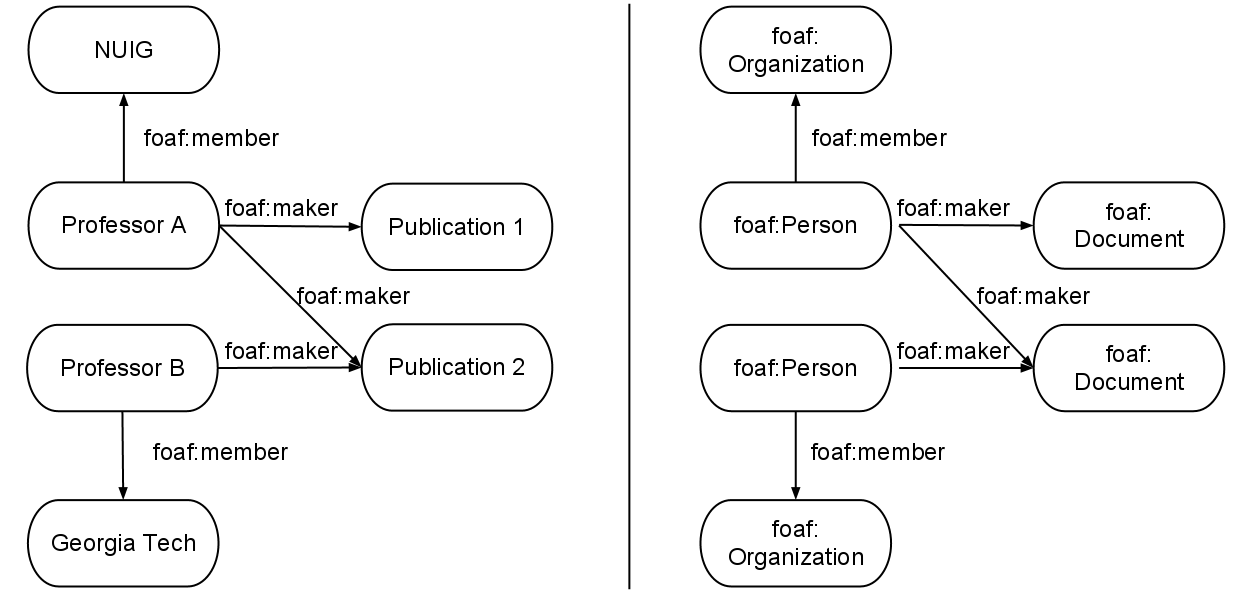
\includegraphics[width=0.75\textwidth]{MergeData.png}
    \caption{Join Relationships and Entity-Class Table}
\end{figure}

\begin{table}[h!]
\begin{center}
  \begin{tabular}{| l | l | l | }
    \hline
    {\bf Subject} & {\bf Predicate} & {\bf Object} \\ \hline    
    Professor A & foaf:maker & Publication 1  \\ \hline
    Professor A & foaf:maker & Publication 2  \\ \hline
    Professor A & foaf:member & NUIG  \\ \hline
    Professor B & foaf:maker & Publication 2  \\ \hline
    Professor B & foaf:member & Georgia Tech  \\ \hline
  \end{tabular}
\end{center}
\caption{Relationship Table}
\end{table}


When performing a join between the tables, we are performing an inner join between the two data sources.  This means an output record is only generated if the key value exists in both tables.  To replace the entities with their class definition an inner join must be performed twice, once to with column values of Entity from the entity-class table and Subject from the relationship table.  This generates an intermediate table, see Table ? below for the academic-dataset.org example.  A second join must be performed with the column values Entity from the entity-class table and Object from the intermediate table.  The result of this operation results in a class-relationship table, Table ? for academic-dataset.org.  Note that the extra fields have already been removed and the table can be represented by Figure 4:Right. The output of this step is the fields: publishing domain, domain of subject, class of subject, property, domain of object, class of object\\

\begin{table}[h!]
\begin{center}
  \begin{tabular}{| l | l | l | l | l | l | }
    \hline
    {\bf Domain} & {\bf Entity} & {\b Class} & {\bf Subject} & {\bf Predicate} & {\bf Object} \\ \hline    
    academic-dataset.org & Professor A & foaf:Person & Professor A & foaf:maker & Publication 1  \\ \hline
    academic-dataset.org & Professor A & foaf:Person & Professor A & foaf:maker & Publication 2  \\ \hline
    academic-dataset.org & Professor A & foaf:Person & Professor A & foaf:member & NUIG  \\ \hline
    academic-dataset.org & Professor B & foaf:Person & Professor B & foaf:maker & Publication 2  \\ \hline
    academic-dataset.org & Professor B & foaf:Person & Professor B & foaf:member & Georgia Tech  \\ \hline
  \end{tabular}
\end{center}
\caption{Intermediate Join Table}
\end{table}

\begin{table}[h!]
\begin{center}
  \begin{tabular}{| l | l | l | l | l | l | }
    \hline
    {\bf Subject Domain} & {\bf Subject Class} & {\b Property} & {\bf Object Domain} & {\bf Object Class}  \\ \hline    
    academic-dataset.org & foaf:Person & foaf:maker & academic-dataset.org & foaf:Document  \\ \hline
    academic-dataset.org & foaf:Person & foaf:maker & academic-dataset.org & foaf:Document  \\ \hline
    academic-dataset.org & foaf:Person & foaf:member & academic-dataset.org & foaf:Organization  \\ \hline
    academic-dataset.org & foaf:Person & foaf:maker & academic-dataset.org & foaf:Document  \\ \hline
    academic-dataset.org & foaf:Person & foaf:member & academic-dataset.org & foaf:Organization  \\ \hline
  \end{tabular}
\end{center}
\caption{Output Table}
\end{table}


\paragraph{Optimizations} \\
In our original implementation, we removed duplicate records from the relationship table. Duplicates were define as having the same subject, predicate, object combination.  Duplicate records imply an entity has multiple relationship to another entity, although the relationship only exists once.  By removing duplicate records the intent was to improve accuracy and reduce the data size. While in reality this operation reduced the reduced the number of record by a mere $3.4\%$.  To reduce the number of comparisons, we moved the removing duplicate operation, over the same fields, to after the class-relationship table was generated.  This reduced the number of records for the unique operation was reduced by 6.35 billion.  

Originally when merging the entity-level relationships with the entity-class table, we first attempted to join the entity-class table with the column Subject from the relationship table, followed by joining on the Object of the relationship table.  After the the inner join on the column Subject, $64.79\%$ of relationships remained.  After joining on the object, only $4.80\%$ of the original relationships remained.  This implied that a maximum of $40.01\%$ of the objects had a class definition.  The key to efficiently computing class-relationship table is to remove as much data as possible as early as possible.  Thus if the inner join was first performed on the column Object from the relationship table and then on the column Subject, this would dramatically reduce the number records to be compared in the second join. A reduction of at least $38.25%$ of the records output from the first inner join.

After performing these optimizations, along with with many others, the computation time reduced from weeks to 37 hours for the entire workflow.  Optimizing the workflow and removing data as early as possible can considerably reduce the computation time. 

\subsubsection{Step 5: Generate Class Super-nodes} 
To complete the class based summary, the nodes of the same class must be aggregated into a single node.  The goal is to transform Figure 4:Right into Figure 2. The class-relationship table output from Step 4 can be used to aggregate nodes of the same class into a single node.  The class-relationship table is grouped by all of its fields and the number of records in each group is counted. This operation produces the count of each relationship between classes.  The result for the academic-dataset.org example is below, the graphical representation is Figure 2.


\begin{table}[h!]
\begin{center}
  \begin{tabular}{| l | l | l | l | l | l | r | }
    \hline
    {\bf Subject Domain} & {\bf Subject Class} & {\bf Property} & {\bf Object Domain} & {\bf Object Class} & {\bf Count}  \\ \hline    
    academic-dataset.org & foaf:Person & foaf:maker & academic-dataset.org & foaf:Document & 3  \\ \hline
    academic-dataset.org & foaf:Person & foaf:member & academic-dataset.org & foaf:Organization & 2  \\ \hline
  \end{tabular}
\end{center}
\caption{Aggregated Relationships}
\end{table}

\subsubsection{Step 6: Convert Unique IDs to Original Values}
During step 1, all data was assigned a unique id.  Now that the graph summary has been completed, the unique ids must be replaced with their original values.  In Hadoop, a MapFile can be used to store unique id and original values and is optimized for fast hash based look up.  After the graph summary has been converted to original values, the workflow is complete.

\subsection{Additional Statistics}
There are many other statistics used within the Sindice Graph Summary, however, not all statistics will be reviewed in detail in this report.  Additional statistics include, the computing the properties of each class super-node and the frequency of properties and classes within a dataset. 



\section{Sindice Assisted SPARQL Editor}
The Sindice Assisted SPARQL Query Editor is a SPARQL query editor which is powered by the Sindice Dataset Summary. The means actual data being queried dictate the editor's recommendations. The assisted editor's interface is shown in Figure 5.  In the toolbar the user can specify a domain in which he would like to query and have recommendations from.  On the right-side of the interface is an options panel that provides a list of classes, properties, and prefixes used with the specified domain.  This allows the user to explore the dataset before or in the process of writing a query.  In the editor box the user can write SPARQL queries and then submit them to the Sindice endpoint.  The results appear in the bottom panel of the interface.  However, the most important feature of the assisted editor is the auto-complete function which will be explained below. 

\begin{figure}
  \centering
    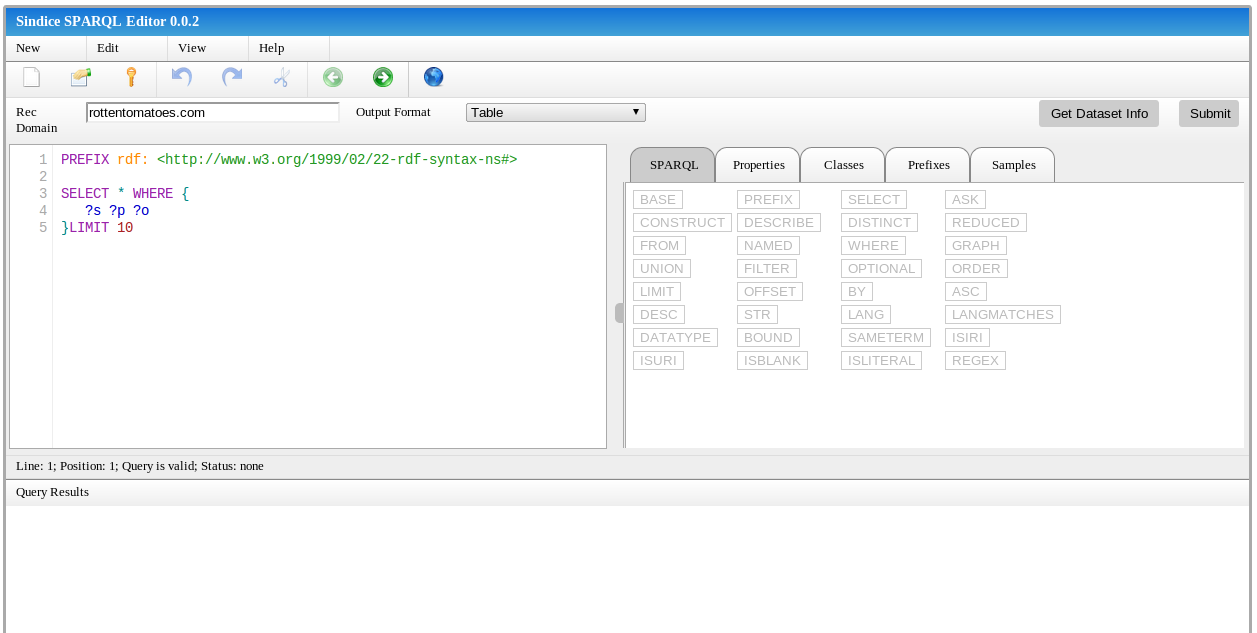
\includegraphics[width=0.95\textwidth]{flint-editor.png}
    \caption{Sindice Assisted SPARQL Query Editor}
\end{figure}

The Sindice Assisted SPARQL Query Editor provides context-aware auto-completion recommendations.  The fundamental model to providing auto-completion recommendations is to use the dataset summary to filter the recommendations, and then to rank the recommendations based on frequency.  For example, if a user specified the academic-dataset.org dataset and requests a recommendation for the following query at the position foaf: .
\begin{table}[h!]
\begin{center}
  \begin{tabular}{| l | }
    \hline
    SELECT * WHERE \{\\  
    \tab ?s a foaf:\\ 
    \}    \\ \hline
  \end{tabular}
\end{center}
\caption{Class Recommendation}
\end{table}
For this query.  The user would be recommended foaf:Person, foaf:Document, and foaf:Document because they are the only classes within the dataset.  The dataset summary can be used to provide the list of all possible recommendations, providing the filter portion of the model.  For the query below, the user would be presented only with foaf:Person because it is the only class within the dataset with the property foaf:member.  The editor can handle much more complex queries, how simple queries were used to introduce the underlying principles.  The editor can also handle OPTIONAL and UNION clauses.

\begin{table}[h!]
\begin{center}
  \begin{tabular}{| l | }
    \hline
    SELECT * WHERE \{\\  
    \tab ?s foaf:member ?org .\\
    \tab ?s a foaf:\\ 
    \}    \\ \hline
  \end{tabular}
\end{center}
\caption{Property Recommendation}
\end{table}

Recommendations are computed in 3 main steps.  First the user's query is parsed, cleaned and analyzed to extract classes and properties.  Second, the extracted information is used to generate a query to extract the possible recommendations from an endpoint containing the Sindice Dataset Summary.  This step also submits the query and obtains the results.  Third is to rank the recommendations using TF-IDF.  




\subsection{Step 1:Parse, Clean, and Analyze Query}
When a user request auto-completion recommendations, the information available to the editor is query, the cursor position, and the specified domain.  To initially parse the query we utilize the Sesame SPARQL Parser, from OpenRDF.org, which represents queries as an abstract syntax tree.  The initial query may contains many superfluous statements.  Examples can include optional statements, unions, branches of unions, and unconnected variables.  This section will not explore the full details of this task, instead choosing to inform the user of the main challenges in completing this task.


\subsubsection{Visitor Definition}
Definition of {\bfAbstract Union Query Tree (UQ-Tree)}.  An UQ-Tree $T$ is a finite set of nodes $N$ with the following properties.\\
1 - Either the set is empty, $T = \phi$; or\\
2 - The set consists of a single containter $r$, $T = \{ r \}$. \\
\\
Definition of {\bf Container}.  A container $C$ is a fininte set of nodes with the following properties.\\
1 - The set contains of a single root node $r$, at most a single query block, and any finite set of distinct unions containers.\\
\\
Definition of {\bf Union Container}.  A union container $U$ is a fininte set of nodes with the following properties.\\
1 - The set consists a single root node $r$ and exactly two distinct containers $C_L$ and $C_R$, $U = \{ r, C_L, C_R \}$ \\
\\
Definition of {\bf Query Block}.  A Query Block $Q$ is single node with the following properties.\\
1 - $Q$ is a leaf node .\\
\\
\\
There exists some function $\nu: X \rightarrow T $, where $X$ is the set of all possible valid SPARQL queries. Thus $\nu$ maps a query $x \in X$ to an UQ-Tree $t \in T$.  $\nu$ has the following properties.\\
1 - Each union $n \in x$ is mapped to a distinct union container $u \in U$.  
2 - If $n$ is a nested union if $n'$ a union and $n \subset n'$.  $n \subset n' \Rightarrow u \subset u'$, where $\nu(n') = u'$. 
3 - The children, $n_L$ and $n_R$ of a union $n \in x$ are mapped to the children $C_L$ and $C_R$ of $u$.  \\
4 - All non union elements $a \in x$ are mapped to query blocks $Q$ such that if $a \in n_v $ then $q \in C_v$, where $\nu(n_v) = C_v$\\
\\
\\
In Dewey Order encoding, each node is assigned a vector that represents the path
from the tree's root to the node and each component of the path represents the local
order of an ancestor node. Using this labelling scheme, structural relationships between
elements can be determined eciently. An element u is an ancestor of an element v if
label(u) is a prefix of label(v). Figure 6.1b depicts a data tree where nodes have been
labelled using Dewey's encoding. Given the label $\<1.1.1.1>$ for the term Renaud, we can
find that its parent is the attribute name, labelled with $\<1.1.1>$ (Cite Renaud's thesis)\\
\\
\\
There exists a function $A(n)$ that results in the set of ancestor nodes for the node $n$.  There also exist a function $P(n)$ that results in the parent node for the node $n$.
\\

\\
{\bf Union Container Pruning Function}\\
First Dewey ordering is applied to T.  Assume the point of focus is contained within a query block $n' \in T$.  There exist some pruning funciton $\epsilon_u$ with the following properties.\\
A node $n \in T$ is pruned if  \\
1 - $n$ is a container, $n \in C$ and \\
2 - $P(n) \in A(n')$ and \\
3 - $n \notin A(n')$ \\
\\
\\
\\

Definition of {\bfAbstract Optional Query Tree (UQ-Tree)}.  An OQ-Tree $P$ is a finite set of nodes $N$ with the following properties.\\
1 - Either the set is empty, $P = \phi$; or\\
2 - The set consists of a single root node $r$ and may contain a single query block and any finite set of distinct optional containers. \\
\\
Defintion of  {\bf Optional Container}.  An Optional Container $O$ is finite set of nodes with the following properties.\\
1 - $O$ consists of a single root node $r$ and may contain a single query block and any finite set of distinct optional containers.\\
\\


There exists some function $\delta: X \rightarrow P $, where $X$ is the set of all possible valid SPARQL queries. Thus $\delta$ maps a query $x \in X$ to an OQ-Tree $p \in P$.  $\nu$ has the following properties.\\
1 - Each union $n \in x$ is mapped to a distinct union container $u \in U$.  
2 - If $n$ is a nested optional if $n'$ a optional and $n \subset n'$.  $n \subset n' \Rightarrow u \subset u'$, where $\delta(n') = u'$. 
3 - The children, $n$ a optiona $n \in x$ are mapped to the children $c$ of $u$.  \\
4 - All non optional elements $a \in x$ are mapped to query blocks $Q$ such that if $a \in n_v $ then $q \in C_v$, where $\delta(n_v) = C_v$\\
\\
\\
{\bf Optional Container Pruning Function}\\
First the root node, $r \in P$ is assigned the identifier $\phi$, the empty set and $\kappa$ is applied to $r$.  Assume the point of focus is contained within a query block $n' \in P$.  There exist some pruning funciton $\epsilon_o$ with the following properties.\\
A node $n \in P$  is pruned if  \\
1 - $n$ is a optional container, $n \in P$, and \\
2 - $n \notin A(n')$\\







\subsubsection{Optional Statements}
Queries may contain optional statements.  However, this does not imply the statements are optional when cleaning the query.   In the example below, the optional statement is truly optional and can be removed from the query.  It does not limit the possible recommendations and only increase the complexity of the generated query.  However, optional statements may not be optional.  If a auto-completion request occurs within an optional statement, all triples within that statement are not optional and must be kept as a hard constraint.  The rule can be summarized as, all optional statements without the auto-complete recommendation cursor can be removed.

\begin{table}[h!]
\begin{center}
  \begin{tabular}{| l | }
    \hline
    SELECT * WHERE \{\\  
    \tab ?s a foaf:\\ 
    \tab OPTIONAL\{ \\
    \tab \tab ?s a foaf:Person \\
    \tab \} \\
    \}    \\ \hline
  \end{tabular}
\end{center}
\caption{Class Recommendation with Optional Statement}
\end{table}
\subsubsection{Union Statements}




\subsubsection{Unconnected Variables}
A query may contain several unconnected variables.  This can increase the complexity of generated query without including additional relevant constraints.  For the example below.  The variable ?s and ?b are completely unconnected.  The means they cannot be connected through a  property nor any path including other variables.  As such, recommendations for the variable ?s are unaffected by the constraints on ?b.  As such, all statements involving ?b can be safely removed.  To fully implement this feature, the editor must check for any connection between entities within the same triple as the auto-complete request and all other entities in the query.  The entities that are unconnected are then removed from the query.

\begin{table}[h!]
\begin{center}
  \begin{tabular}{| l | }
    \hline
    SELECT * WHERE \{\\  
    \tab ?s a foaf:Document .\\ 
    \tab ?s foaf: \\
    \tab ?b a foaf:Document.\\ 
    \}    \\ \hline
  \end{tabular}
\end{center}
\caption{Property Recommendation with Classes}
\end{table}

\subsection{Step 2: Obtain Recommendations}
Using the Sindice Dataset Summary, it is possible to find all possible recommendations.  This is performed by translating the cleaned query into a query for the dataset summary.  This is dependent on the RDF representation of the dataset summary.  The RDF representation of the dataset summary will not be introduced in this paper, however, a note on difficulties we encountered will be provided below.  The dataset summary cannot be used to filter recommendations based on literal values as it does not contain this information.  It can, however, filter the results based on if an entity has that property.  The dataset summary cannot guarantee that the query will not result in zero records.  The dataset summary contains information concerning classes and does not guarantee that every entity belonging a class has all of its properties.  As such it is still possible to write a valid query that has no results.

\subsubsection{RDF Representation}
Note about the need for properties and relationships to be modeled the same


\subsection{Step 3: Rank Recommendations}

After the possible recommendations have been obtained from step.  The results must be ranked.  To rank the recommendations, we use a TF-IDF implementation as defined by equation 1.

\begin{equation}
idf(t) = \log{\frac{\mid D \mid}{ \mid \left \{ d : t \in d  \right \} \mid }}
\end{equation}

\begin{equation}
tfidf(t,d) = tf(t,d) \times idf(d)
\end{equation}

where $\mid D \mid$ is the number of datasets and $\mid \left \{ d : t \in d  \right \} \mid$ is the number of domains that contain the class or property. When recommending a class, $tf(t,d)$ is the number of instances of that class definition or property $t$ within the dataset $d$ divided by the total entities, if $t$ is a class, or the total number of properties within $d$, if $t$ is a property. The results are sorted in descending order and only the top N results are returned to the user.

\section{Discussion and Future Work}
Future work\\
Improve editor interface, cross-dataset queries. Empirical Evaluation of Editor.  Formal algebra of summary. Full-text search Improved ranking.\\  
SPARQL-based summary to integrate with editor for small datasets\\
CONCLUSION\\
Optimization essential for workflow\\\
Graph summary easier to process, useful in many applications, easier to write queries\\


\end{document}
